\chapter{PENDAHULUAN}\label{pendahuluan}


\section{Latar Belakang}\label{subBab:latar belakang}
Indonesia adalah sebuah negara adi kuasa di bidang budaya. Begitulah ungkapan Fransesco Bandarin selaku Asisten Dirjen UNESCO (\textit{United Nations Educational, Scientific, and Cultural Organization}) Bidang Budaya pada sidang UNESCO ke-39 di Paris tahun 2017 \cite{statistikBudaya}. Bagaimana tidak, Indonesia merupakan rumah bagi 1.340 suku bangsa dengan 2.500 jenis bahasa, serta kekayaan warisan budaya baik benda maupun tak benda yang jumlahnya mencapai ribuan. Salah satu bentuk warisan budaya Indonesia yang cukup menarik adalah seni musik tradisional. Musik tradisional lahir dan berkembang dari budaya daerah tertentu dan diwariskan secara turun-temurun \cite{bukuMusik}. Seni musik tradisional memiliki beberapa unsur penyusun, salah satu yang terpenting adalah alat musik tradisional \cite{webKemendikbud}. \par 
Keanekaragaman budaya Indonesia juga tercermin pada alat musik tradisional. Setiap daerah memiliki alat musik tradisionalnya masing-masing. Sebagai contoh, daerah Wonosobo di Jawa Tengah memiliki alat musik bernama \textit{bundengan} (Gambar \ref{fig:bundengan}). Berdasarkan dokumentasi awal yang dilakukan oleh Kunst pada tahun 1949, alat musik ini pada awalnya disebut \textit{kowangan}, sebuah anyaman bilah bambu yang disusun seperti perisai. \textit{Kowangan} digunakan sebagai pelindung kepala dari panas dan hujan oleh para penggembala bebek \cite{kunst}. Ketika sedang menunggu bebeknya yang sedang makan, mereka akan duduk di bawah \textit{kowangan} dan menghibur diri mereka sendiri dengan memainkan lagu-lagu tradisional \cite{skripsiSaid}. Para penggembala bebek bermain musik menggunakan \textit{kowangan} dengan cara memasangkan senar dan bilah bambu (Gambar \ref{fig:bilahBambu}) pada bagian dalam \textit{kowangan}. Selain itu, pada senar yang terpasang juga disematkan potongan ranting bambu yang disebut \textit{bandulan} (Gambar \ref{fig:senarBandulan}). Gambar \ref{fig:kowanganKunst} memperlihatkan bagaimana \textit{kowangan} digunakan sebagai pelindung kepala dan dimainkan oleh para penggembala bebek. Ketika \textit{kowangan} berubah fungsinya menjadi sebuah instrumen musik, benda ini tidak lagi disebut sebagai \textit{kowangan}, melainkan sesuatu yang benar-benar baru: \textit{bundengan} \cite{palmer}. \par  
\begin{figure}[t!]
    \centering
    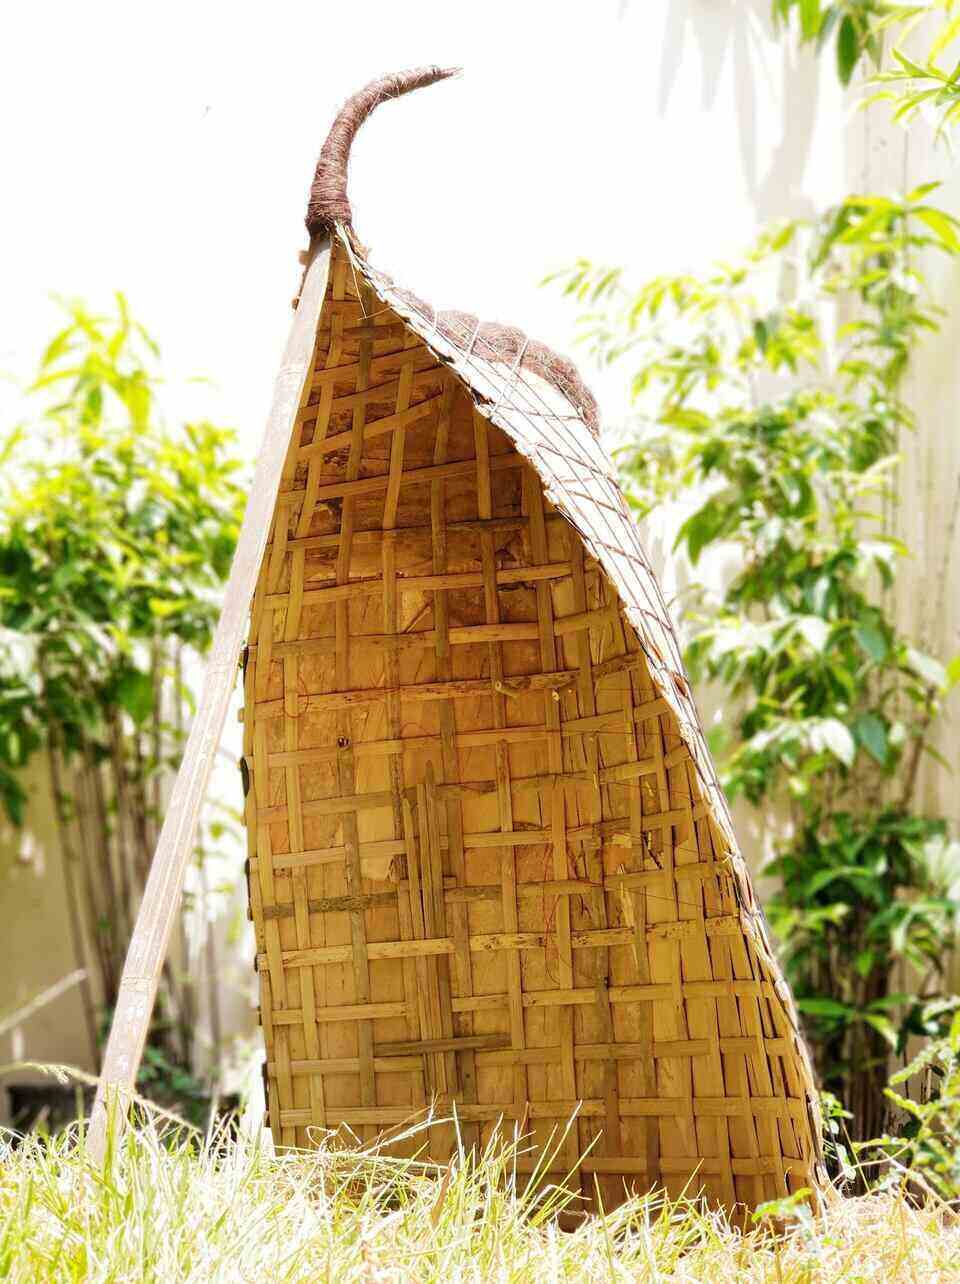
\includegraphics[width=7 cm]{Gambar/bundengan_full.jpg}
    \caption{Alat musik tradisional \textit{bundengan} \cite{fotoBuAri}.}
    \label{fig:bundengan}
\end{figure}
\begin{figure}[h!]
    \centering
    \subfigure[]{\label{fig:bilahBambu}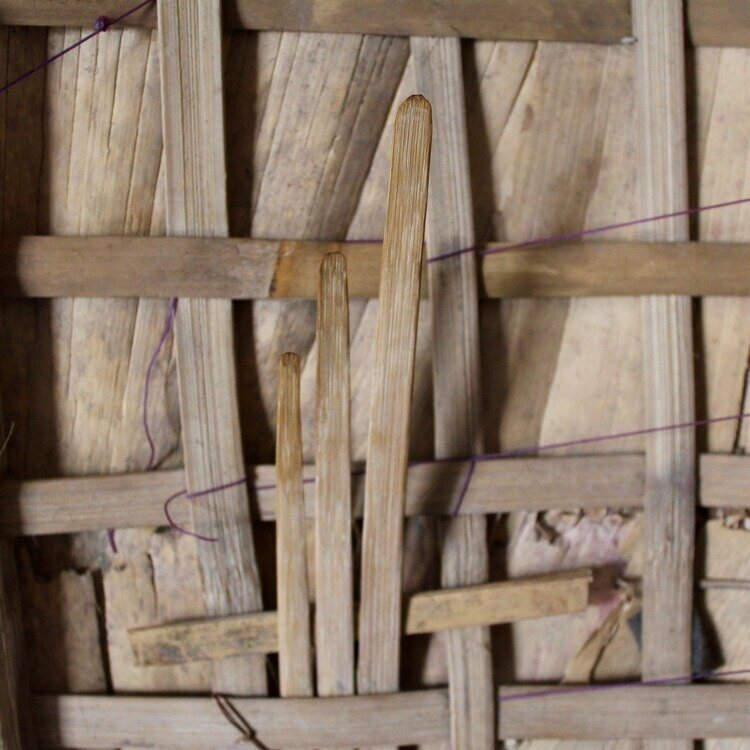
\includegraphics[width=45mm]{Gambar/pelat-bambu.jpg}}
    \hspace{1cm}
    \subfigure[]{\label{fig:senarBandulan}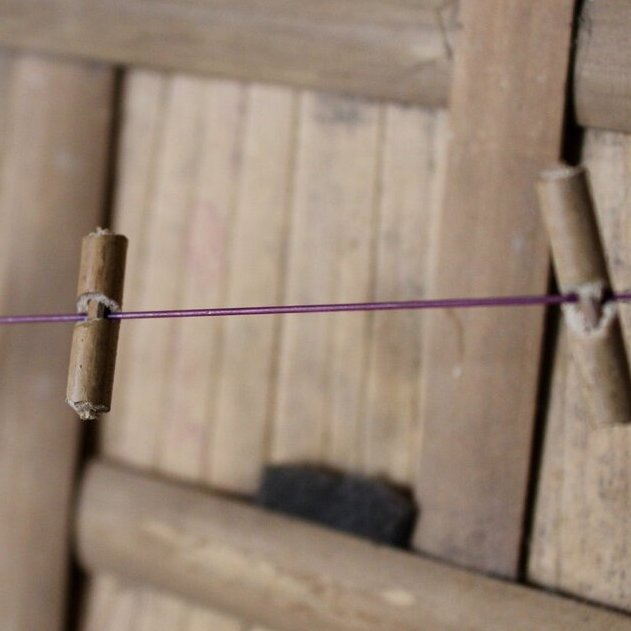
\includegraphics[width=45mm]{Gambar/senar-bandulan.jpg}}
    \caption{Beberapa bagian \textit{bundengan} selain \textit{kowangan}; (a) pelat bambu dan (b) senar dengan \textit{bandulan} \cite{palmer}.}
\end{figure}
\begin{figure}[t!]
    \centering     %%% not \center
    \subfigure[]{\label{fig:PelindungKepala}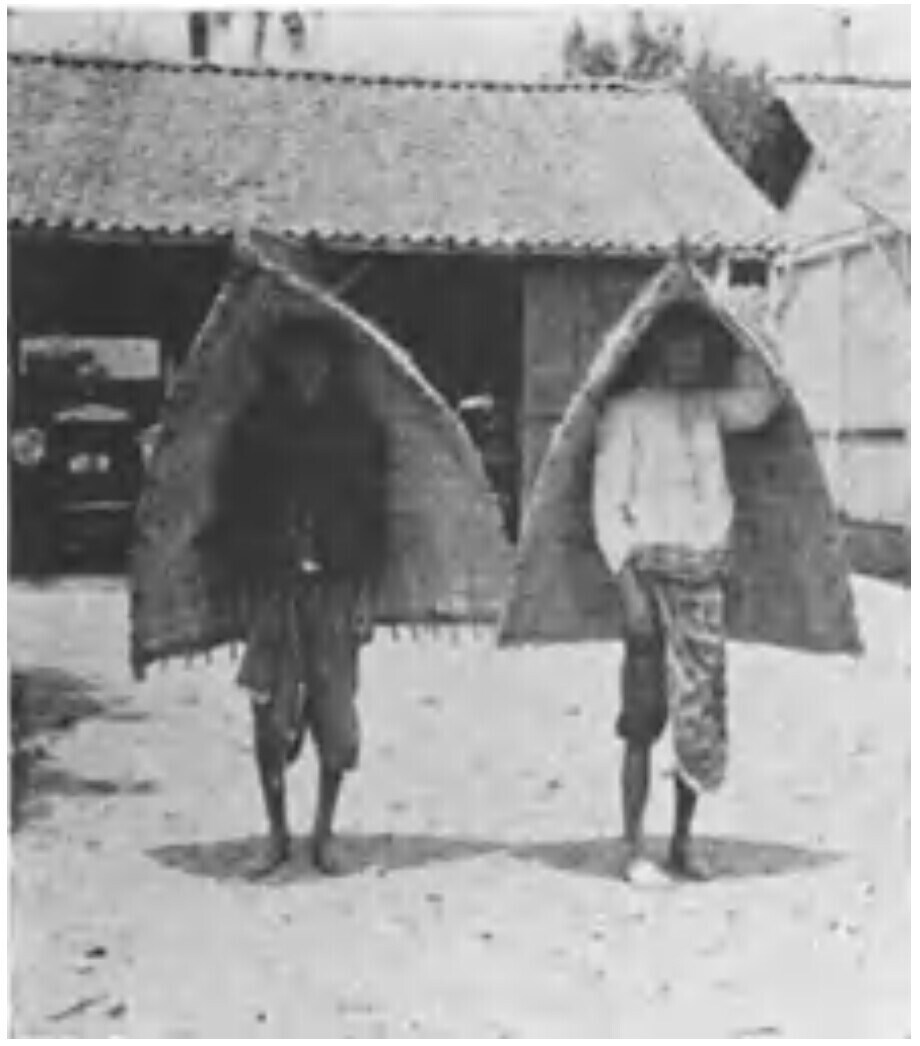
\includegraphics[width=50mm]{Gambar/Kowangan_PelindungKepala.jpg}}
    \hspace{1cm}
    \subfigure[]{\label{fig:KowanganDimainkan}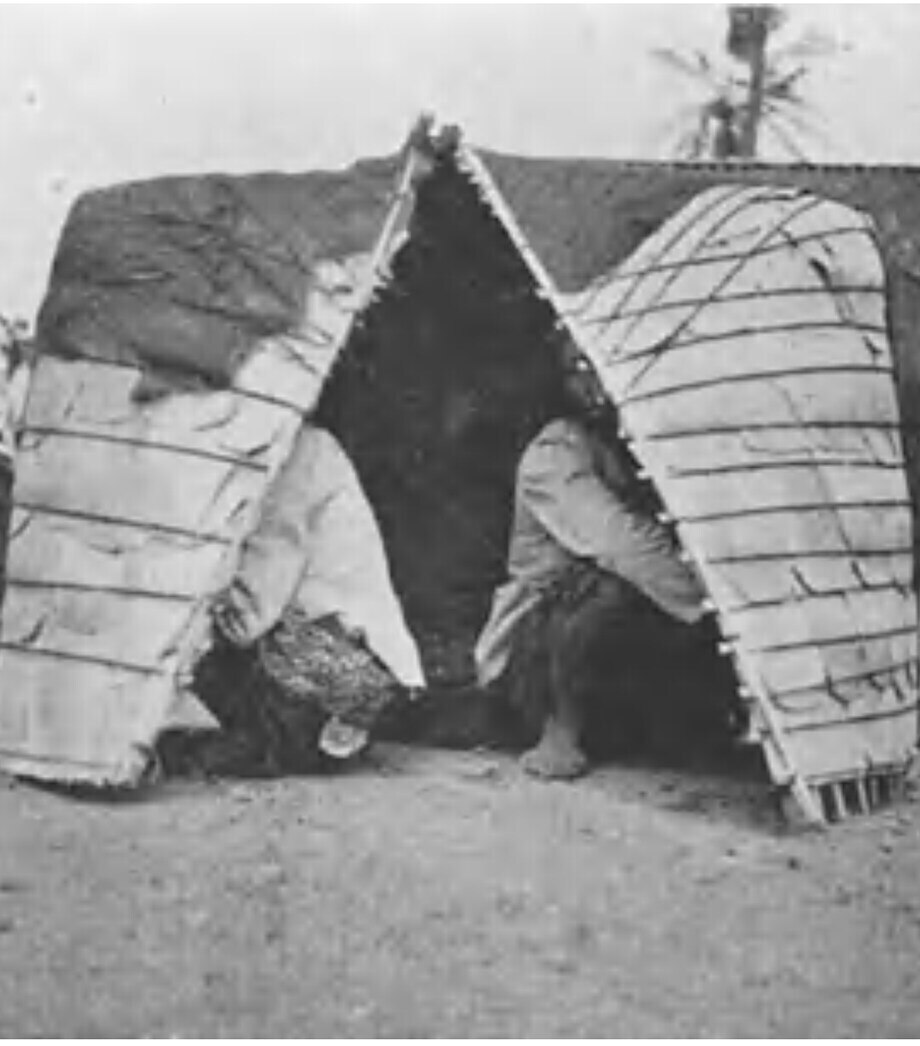
\includegraphics[width=50mm]{Gambar/KowanganDimainkan.jpg}}
    \caption{Penggembala bebek sedang (a) menggunakan \textit{kowangan} sebagai pelindung kepala dan (b) memainkan \textit{kowangan}  \cite{kunst}.}
    \label{fig:kowanganKunst}
\end{figure}
\newpage
Seiring dengan berkembangnya zaman, profesi penggembala bebek semakin berkurang. Akibatnya, eksistensi \textit{bundengan} juga terancam punah \cite{prosidingDirektivitas}. Berbagai upaya dilakukan dalam rangka menjaga kelestarian \textit{bundengan}, seperti menghadirkan \textit{bundengan} pada pembelajaran di lingkup sekolah formal. Bukti nyata dari upaya ini dapat ditemukan di SMP Negeri 2 Selomerto, Kabupaten Wonosobo \cite{skripsiSaid}. Siswa-siswi di sekolah tersebut diajak untuk mengenal musik \textit{bundengan} sebagai ciri khas kedaerahan oleh guru seninya. Selain sebagai sarana pembelajaran, \textit{bundengan} juga kerap dihadirkan sebagai sarana pertunjukan. Pertunjukan yang dimaksud adalah ditempatkannya permainan musik \textit{bundengan} di ruang pementasan dan dipertontonkan ke khalayak umum. Pementasan bundengan biasanya dilakukan pada acara karnaval budaya, festival, pentas seni tradisional, atau undangan hajatan masyarakat \cite{skripsiSaid}. Gambar \ref{fig:konserBundengan} memperlihatkan salah satu pementasan \textit{bundengan}. \par
\begin{figure}[t!]
    \centering
    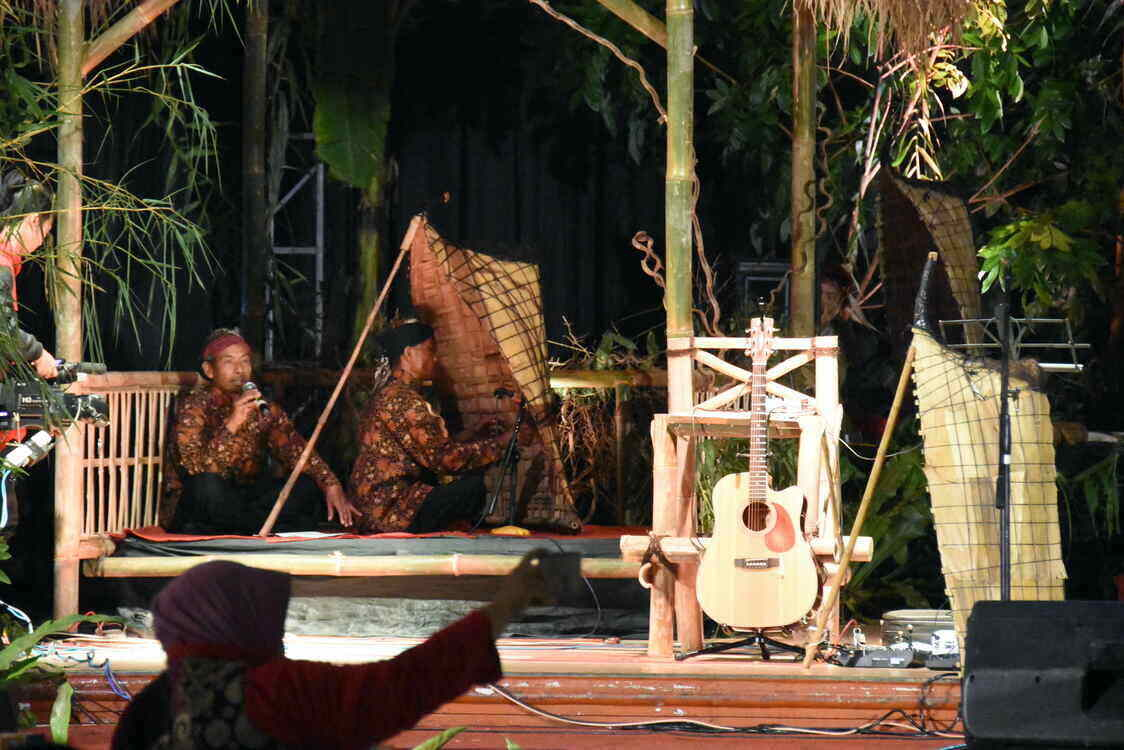
\includegraphics[width=9.5cm]{Gambar/Pentas Bundengan.jpg}
    \caption{Pementasan \textit{bundengan} \cite{pentasBundengan}.}
    \label{fig:konserBundengan}
\end{figure}
Sayangnya, upaya konservasi \textit{bundengan} melalui pementasan panggung tidak berjalan dengan baik. Musik yang dihasilkan oleh \textit{bundengan} berasal dari bunyi petikan senar dan bilah bambu. Senar dan bilah bambu ini terpasang pada struktur utama \textit{bundengan}, yakni \textit{kowangan}. Bentuk dan struktur dari \textit{kowangan} mengakibatkan bunyi yang dihasilkan senar dan bilah bambu terfokus pada area yang diselimuti oleh \textit{kowangan} \cite{alatMusikPersonal}. Hal ini menyebabkan pengalaman terbaik dalam mendengarkan musik \textit{bundengan} berada pada posisi pemain, sehingga para pendengar dalam pementasan \textit{bundengan} akan mendapatkan kualitas musik yang kurang maksimal. Untuk mengatasi masalah ini, musisi \textit{bundengan} telah mencoba menggunakan pengeras suara, namun bunyi yang diterima pendengar tidak sesuai dengan bunyi asli dari \bundengan seperti yang dinikmati oleh musisi yang duduk di bawah \textit{kowangan} \cite{alatMusikPersonal}. Memang, jika meninjau kembali bagaimana \textit{bundengan} diciptakan, alat musik ini hanya hadir sebagai alat musik untuk menghibur diri sang pemain \cite{palmer2}. \par 




\section{Perumusan Masalah}\label{subBab:rumusanMasalah}
Pementasan \textit{bundengan} membantu memperkenalkan \textit{bundengan} kepada masyarakat umum. Langkah ini sangat tepat sebagai upaya konservasi dari alat musik \textit{bundengan}. Oleh sebab itu, masalah mengenai kualitas musik \textit{bundengan} saat pementasan panggung akan menghambat terlaksananya konservasi \textit{bundengan}. Masalah teknis ini tidak hanya perlu dihadapi oleh musisi dan pegiat \textit{bundengan} saja, namun juga perlu dihadapi oleh para insinyur di Indonesia. \par 
Pementasan musik dapat dikatakan ideal ketika pendengar dapat mendengar dengan jelas musik yang sedang dimainkan. Dengan kata lain, pendengar dapat merasakan dengan jelas setiap nada yang dimainkan. Setiap pendengar memiliki persepsi yang berbeda terhadap tingkat kekerasan bunyi alat musik yang dimainkan maka untuk mengukurnya secara objektif digunakan besaran yang disebut TTB (Tingkat Tekanan Bunyi). TTB didefinisikan sebagai tingkat fluktuasi tekanan udara yang disebabkan oleh sumber bunyi \cite{meyer}. Perubahan tekanan ini merambat melalui ruang dalam bentuk gelombang. Ketika sampai di telinga, fluktuasi tekanan ini diterjemahkan menjadi sebuah bunyi. Tingkat perbedaan tekanan ini menentukan seberapa keras bunyi yang dirasakan oleh telinga. \par 
Setiap sumber bunyi menghasilkan gelombang bunyi yang merambat dalam ruang. Meskipun demikian, intensitas bunyi yang dihasilkan tidak selalu sama untuk setiap arah rambatnya. Fenomena ketergantungan nilai TTB terhadap arah rambat ini dikenal dengan istilah karakteristik direksional atau direktivitas \cite{meyer}. Pada Gambar \ref{fig:diagramPolarBiola} diperlihatkan pola direktivitas dari salah satu nada biola. Gambar \ref{fig:diagramPolarBiola} juga memperlihatkan pola direktivitas derau dengan frekuensi pusat yang sama dengan nada biola tersebut. Pola direktivitas tersebut ditampilkan dalam diagram polar. Radius dari diagram polar mewakili besarnya nilai TTB yang berkisar antara 0 dB sampai 40 dB. Dapat dilihat bahwa untuk arah 220º-300º bunyi dari nada biola tidak dapat didengar karena tertutup oleh derau. \par 
Posisi pemain \textit{bundengan} dan pendengar yang berbeda tentu memiliki kemungkinan perbedaan kualitas musik yang diterima. Karena masalah yang dihadapi adalah kualitas musik \textit{bundengan} yang kurang baik pada posisi penonton maka untuk menentukan solusi dari masalah ini perlu terlebih dahulu dipahami bagaimana direktivitas dari alat musik \textit{bundengan}. \par 

\begin{figure}[t!]
    \centering
    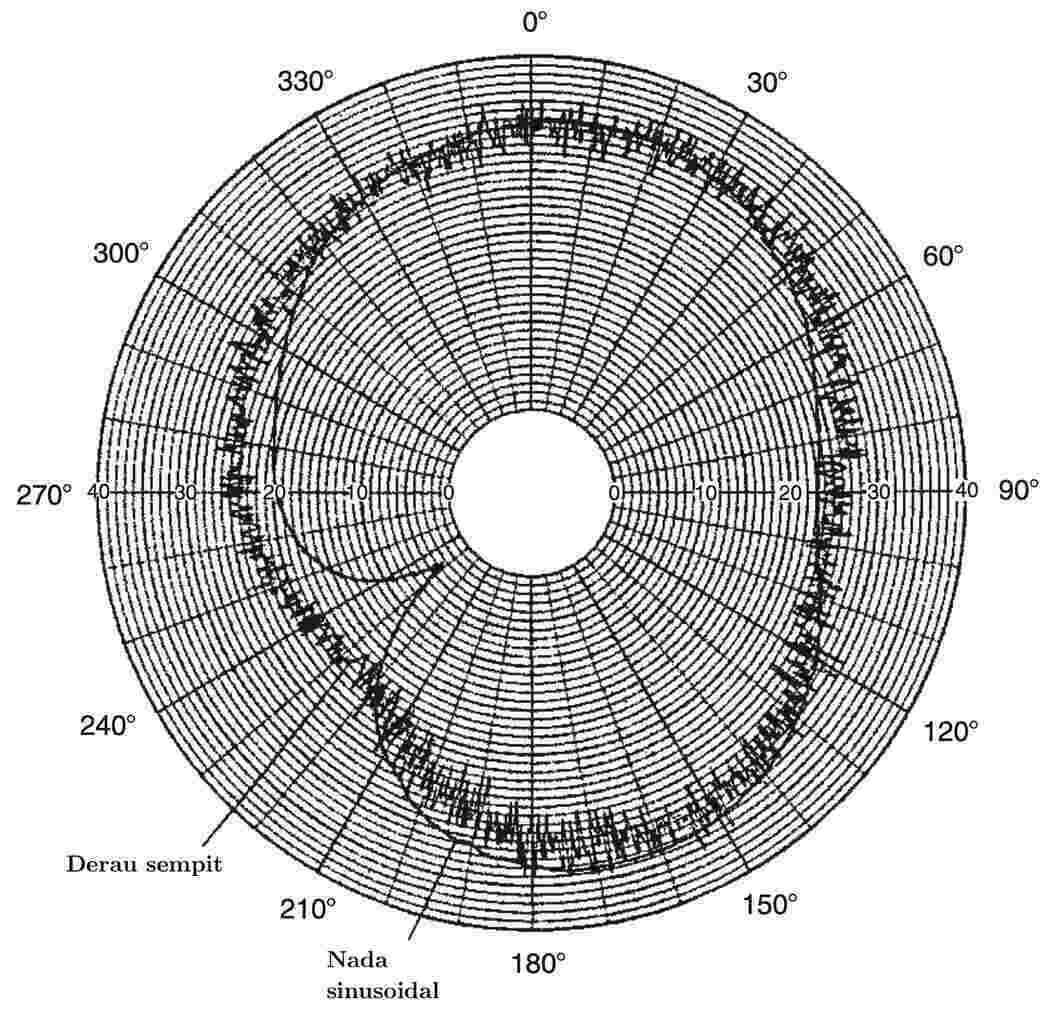
\includegraphics[width=11cm]{Gambar/diagramPolarBiola.jpg}
    \caption{Perbandingan direktivitas sebuah biola pada frekuensi 1.250 Hz dan derau sempit dengan frekuensi pusat 1.250 Hz \cite{meyer}.}
    \label{fig:diagramPolarBiola}
\end{figure}
\newpage
Dalam konteks pementasan \textit{bundengan}, data direktivitas telah berhasil diperoleh. Meskipun begitu, pengaplikasian dari data direktivitas tersebut belum dapat terlaksana. Hingga saat ini, data direktivitas yang diperoleh sulit untuk dipahami oleh kalangan musisi maupun pegiat \textit{bundengan}. Pasalnya data ini ditampilkan dalam bentuk yang maknanya masih sulit dipahami. Pada Gambar \ref{fig:contohDataDirektivitas} diperlihatkan salah satu hasil olah data direktivitas \bundengan yang telah diukur. Hasil olah data tersebut memperlihatkan perbedaan warna sebagai perbedaan nilai TTB untuk setiap variasi nilai frekuensi (sumbu mendatar) dan arah rambat bunyinya (sumbu tegak). Dengan data ini sebetulnya sudah dapat diketahui nilai TTB untuk setiap arah dan frekuensi tertentu. Namun, dari sudut pandang musisi dan pegiat \bundengan bentuk penyajian data yang kompleks ini cukup sulit dimengerti. \par 
\begin{figure}[t!]
    \centering
    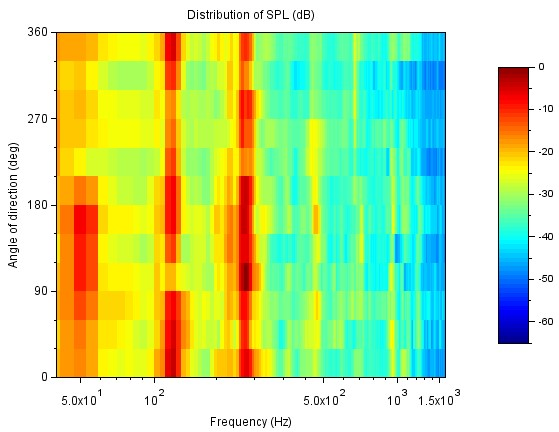
\includegraphics[width=10cm]{Gambar/contohDataDirektivitas.jpg}
    \caption{Hasil olah data direktivitas bunyi salah satu senar \bundengan \cite{prosidingDirektivitas}.}
    \label{fig:contohDataDirektivitas}
\end{figure}

Penyampaian informasi dapat dilakukan dengan berbagai cara, lisan maupun tulisan. Manusia pada dasarnya adalah makhluk hidup yang menggunakan penglihatan sebagai indera utama untuk memperoleh informasi. Visualisasi adalah metode penyampaian informasi menggunakan representasi secara grafis. Terkadang, penyampaian informasi menggunakan satu halaman tulisan ataupun beberapa kalimat lisan tidak efektif digunakan dalam menyampaikan informasi yang kompleks. Sebuah gambar dapat mengandung lebih banyak informasi dan dapat diproses lebih cepat dibanding satu halaman kata-kata. Ini karena interpretasi gambar dilakukan secara paralel dalam sistem persepsi manusia, sementara kecepatan analisis teks dibatasi oleh proses membaca yang berurutan \cite{buku_visual}. Dalam ranah musik, sebetulnya para komposer dan musisi telah cukup lama menggunakan visualisasi. Sebagai contoh, Gambar \ref{fig:gundulPacul} memperlihatkan penggalan notasi musik lagu "Gundul Pacul". Notasi musik merupakan kumpulan simbol tertulis yang merepresentasikan suara musik \cite{bukuTeoriMusik}. Dengan notasi tersebut, komposer dapat menyampaikan kepada musisi tentang nada apa yang harus dimainkan dan kapan harus memainkannya \cite{videoTedEd}. \par  
\begin{figure}[t!]
    \centering
    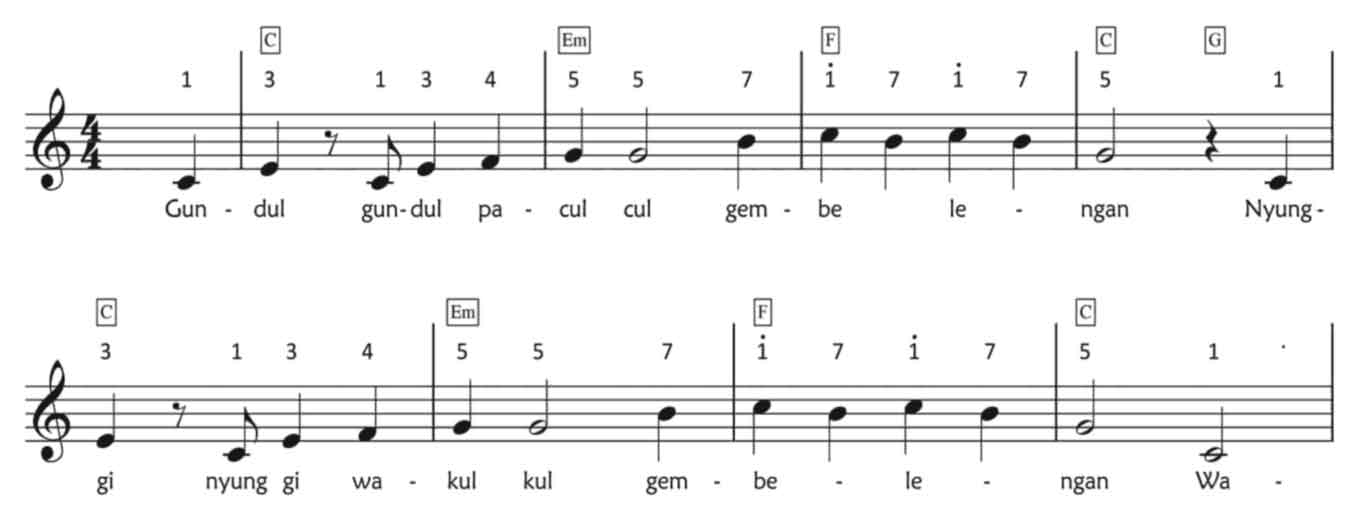
\includegraphics[width= 14 cm]{Gambar/gundulPacul.jpg}
    \caption{Penggalan notasi musik lagu "Gundul Pacul" \cite{bukuLaguIndo}.}
    \label{fig:gundulPacul}
\end{figure}
Kemudahan memproses informasi juga dapat diterapkan pada data direktivitas \textit{bundengan}. Salah satu penyebab belum terciptanya pementasan \bundengan yang baik adalah karena hasil pengukuran data direktivitas tidak ditampilkan dalam bentuk yang mudah dipahami musisi dan pegiat \textit{bundengan}. Oleh karena itu, diperlukan sebuah sistem yang dapat memvisualisasikan data direktivitas \bundengan secara lebih interaktif. Sistem ini perlu dapat memenuhi kebutuhan para musisi dan pegiat \bundengan dalam merancang pementasan \bundengan yang lebih baik. Untuk mengetahui kebutuhan tersebut telah tercapai atau belum maka kinerja sistem ini perlu dianalisis \cite{bukuUlrich}. \par 


\section{Batasan Masalah}
\begin{enumerate}
    \item Data yang digunakan adalah data direktivitas dua buah \textit{bundengan}. \textit{Bundengan} pertama dibuat oleh pengrajin senior dengan empat senar, sedangkan \textit{bundengan} kedua dibuat oleh pengrajin muda dengan delapan senar.
    \item Data ini berasal dari pengukuran bunyi setiap senar \textit{bundengan} menggunakan tujuh mikrofon kondensor yang disusun setengah lingkaran pada setiap sudut 30º, seperti yang ditunjukkan pada Gambar \ref{fig:bundenganBatasanMasalah}.
    \item Interaksi gelombang bunyi dengan obyek sekitar dapat diabaikan karena pengukuran dilakukan di dalam sebuah ruangan \textit{semi-anechoic}.
    \begin{figure}[h!]
        \centering
        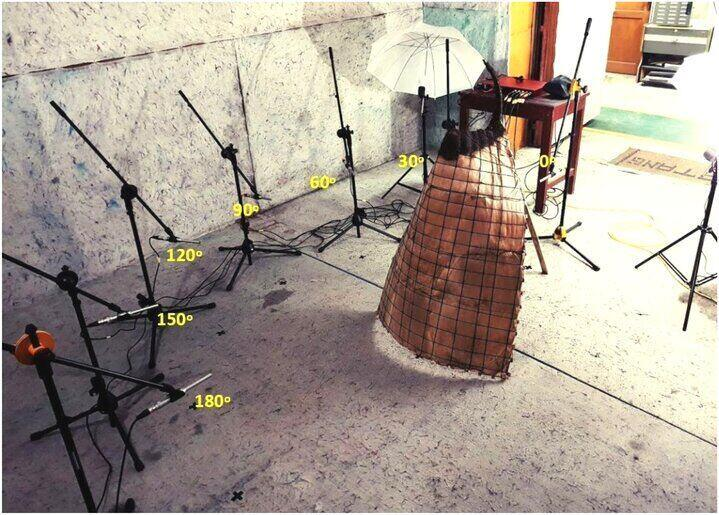
\includegraphics[width=10 cm]{Gambar/bundenganBatasanMasalah.jpg}
        \caption{Penyusunan \textit{bundengan} dan perlengkapan dalam pengukuran data direktivitas \textit{bundengan} \cite{prosidingDirektivitas}.}
        \label{fig:bundenganBatasanMasalah}
    \end{figure}
\end{enumerate}


\section{Tujuan}
\begin{enumerate}
    \item Membangun sebuah sistem visualisasi interaktif data direktivitas \textit{bundengan} yang sesuai dengan kebutuhan untuk merancang pementasan \textit{bundengan} menjadi lebih baik.
    \item Menganalisis kinerja sistem visualisasi interaktif data direktivitas \textit{bundengan}.
\end{enumerate}


\section{Manfaat}
Penelitian ini akan bermanfaat untuk dua bidang, yaitu: \par 
\begin{enumerate}
    \item Penelitian ini bermanfaat untuk bidang kebudayaan. Dalam rangka membantu konservasi \textit{bundengan}, penelitian ini memudahkan musisi \textit{bundengan} memahami direktivitas \textit{bundengan}. Pemahaman ini kemudian dapat dijadikan dasar pada perancangan pementasan \textit{bundengan} yang lebih baik, yaitu menciptakan pementasan \textit{bundengan} di mana kualitas musik yang diterima pendengar adalah yang paling maksimal.
    \item Selain itu, penelitian ini juga bermanfaat untuk bidang rekayasa, khususnya ilmu akustika. Konsep dan metode yang digunakan dalam penyampaian data direktivitas pada penelitian ini dapat dimanfaatkan insinyur akustika lain untuk kemudian dikembangkan dan diterapkan pada data akustika lain yang menyangkut kebutuhan pemahaman musisi dan pegiat musik. 
\end{enumerate}